\documentclass[a4paper]{sbgames}               % final
\usepackage{times}
\usepackage{graphicx}

\usepackage[utf8]{inputenc}
\usepackage[T1]{fontenc}
\usepackage{tikz}
\usepackage{algorithm}
\usepackage{algpseudocode}
\usepackage{pifont}


%% use this for zero \parindent and non-zero \parskip, intelligently.
\usepackage{parskip}

%% the 'caption' package provides a nicer-looking replacement
\usepackage[labelfont=bf,textfont=it]{caption}

\usepackage{url}

%% Paper title.
\title{A modular GPU raytracer using OpenCL for non-interactive graphics}

%% Author and Affiliation (multiple authors). Use: and between authors

\author{Henrique Nunes Jung\\ Univesidade do Vale do Rio dos Sinos
}
\contactinfo{\{henriquenj\}@gmail.com
}
%% Keywords that describe your work.
\keywords{GPGPU, OpenCL, computer graphics, raytracing}

%% Start of the paper
% Attention: As you need to insert EPS images in Postscript,
% you need to insert PDF images into PDFs.
% In the text, extensions cancbe omitted (latex use .eps, pdflatex get .pdf)
% To convert them: epstopdf myimage.eps
\begin{document}

\teaser{

}

%% The ``\maketitle'' command must be the first command after the
%% ``\begin{document}'' command. It prepares and prints the title block.

\maketitle

%% Abstract section.

\begin{abstract}

  In this paper we describe the implementation of a modular
  plug-in-based raytracer renderer called \emph{RenderGirl} suitable
  for running inside the OpenCL framework. RenderGirl is split between
  two main portions: Core and Interface, where Core portions provides
  the bulk of raytracing operations and manages the communication with
  OpenCL; and interfaces provides communication with a given
  host program. In order to validate the plugin architecture, we
  implemented an interface using Blender as host program. The initial
  target market for this software is architects interested in using
  GPUs and other OpenCL-compatible hardware for model
  visualization. Accelerations structures were used to increase the
  robustness of the renderer and decrease rendering times.
  % TODO: add details about which accelerations structures
\end{abstract}

%% The ``\keywordlist'' command prints out the keywords.
\keywordlist
\contactlist

\section{Introduction}

Platforms for general purpose computing using GPUs started when
NVIDIA\footnote{NVIDIA website \url{http://www.nvidia.com/}} released
its GPGPU platform called CUDA\footnote{CUDA homepage
 \url{http://www.nvidia.com/object/cuda_home_new.html}}, which is
capable of running only on NVIDIA hardware. OpenCL\footnote{OpenCL on
 Khronos Group website \url{https://www.khronos.org/opencl/}} was
born sometime later using the label \emph{heteregenous computing}, in
order to specifies that the platform was supported by many kinds of
hardware and computers processors, including CPUs and non-NVIDIA GPUs,
which could be implemented by any vendor interested in developing
hardware focused on parallel computation.

Within this context, this work aims to provide a modular plugin-based
raytracer software that takes advantage of the parallel capabilities
of modern GPUs while maintaing hardware agnosticism by using the
portability OpenCL provides to hardware vendors and developers. By
being modular, it's also capable of running inside larger 3D suites
such as Blender, this way we can delegate other tasks to the host 3D
program and focuses on the rendering tasks.
% TODO: add here the method of BVH once it's selected

We propose a C++ application with wrappers for
Python %TODO: do I really need a python wrapper?
and C++ and a reference plugin for Blender, used to validate the
plugin architecture. The code has only portable system calls and
OpenCL function calls. In order to guarantee compilation on multiples
compilers, CMake was used as build system. Development happens on
GitHub, which contains the code, issue tracker and
documentation.

Intrinsic problems that arrives with GPU raytracing includes the cost
of synchronizing and stoping working threads, poor branch prediction,
high latency of different OpenCL memory models, high latency on the
bus used between GPU and main memory (usually PCI Express) and the
broad variety of GPUs and OpenCL capable hardware, which can generate
different results on different setups.
% TODO add benefits of programming using GPUs, start with "by contrast"
% TODO find source for this

There are several acceleration structures for increase the efficiency
of rendering, which are called \emph{spatial data structures}. Some of
these structures are \emph{bounding volume hierarchies} (BVH),
\emph{binary space partioning}, trees, quadtrees and octrees. They
hierarchically subdived a scene so the queries for the objects become
faster \cite[Chapter~14]{akenine-moller:2008}. Non real-time renderers
do not have these constraints and therefore can employ expensive
algorithms, generating images of higher quality, while taking
advantage of the spatial structures in order to speed up
operations. This is the case for our work.

\section{Related Work}
\label{sec:related-work}

Applications that provides GPU rendering capabilities for
non-interactive graphics include Blender Cycles\footnote{Cycles
  website \url{http://www.blender.org/manual/render/cycles/}} , Octane
render \footnote{Octane website
  \url{https://home.otoy.com/render/octane-render/}}, V-Ray renderer
\footnote{VRAY website
  \url{http://www.chaosgroup.com/en/2/vray.html}}, Redshift
\footnote{Redshift website
  \url{https://www.redshift3d.com/products/redshift}} and Indigo
renderer \footnote{Indigo website
  \url{http://www.indigorenderer.com/}}. Indigo and Cycles claims to
run using the OpenCL framework. Cycles is the only one that is free
software; originally it only supported CUDA-capable devices, but newer
versions of Blender ship with Cycles that works with limited features
also on OpenCL, although the developers specifies that CUDA platform
is more mature \footnote{Cycles GPU rendering page
  \url{http://www.blender.org/manual/render/cycles/gpu_rendering.html}}.
Also Cycles takes a different approach for device abstraction by
performing \emph{platform abstraction} by issuing commands to a common
\emph{device interface} that can redirect function calls to CUDA,
OpenCL, CPU or network; although the latter is still experimental
\footnote{Blender Cycles Developer Documentation
  \url{http://wiki.blender.org/index.php/Dev:2.6/Source/Render/Cycles/Devices}}. Our
work delegate the device abstraction entirely to OpenCL.

Recent related work on the computing literature includes: Áfra and
Szirmay-Kalos propose a novel traversal algorithm for BVH that doesn't
uses a stack, and can execute both on CPU and GPU platforms. They
introduce the concept of \emph{bitstack}, which is an integer used in
the place of a stack \cite{Afra}. Kalajanov and colleagues propose an
acceleration structure using hierarchical two-level grids implemented
in CUDA, which can eliminated problems arriving from using a single
uniform grid for subdividing a scene. They call "teapot in a stadium
problem", where a great amount of objects is allocated on a single
cell of the uniform grid \cite{Kalojanov}. Ravichandran and colleagues
proposes a parallel divide and conquer raytracing suited for
GPUs. Divide and conquer ray tracing remove the need of creating an
explicit aceleration structures once per frame, instead it creates an
aproximation using bound boxes \cite{Ravichandran}. Shumskiy and
Parshin write a comparative study of ray-triangle intersection
algorithms, how they perform on GPU hardware and how BVH acceleration
structures can be optimized for each one. They point out that some of
their results differs from generation to generation of the same line
of GPUS due to change in the micro-architecture.
% TODO: this last sentece should go to other section, more specific
\cite{Shumskiy}. Wong and colleagues propose an optimizatin method for
GPU ray tracing by dividing objects into view-sets based on light and
camera position, the BVH is then built using these views-sets, this
way the amount of triangles on the BVH is reduced \cite{Wong}. Widmer
and colleagues proposes efficient acceleration structure for real-time
screen space raytracing, they use an hybrid data structure combining
BVH and local planar approximation \cite{Widmer}. A great portion of
these works deal with acceleration structures for GPU raytracing -
e.g. kd-trees, BVHs -, which indicates the complexity of these
structures on GPU hardware.

\subsection{Contextualization}

Our own implementation relies on ray-triangle intersection algorithm
developed by Möller and Trumbore that aims to be fast by avoiding
ray-plane intersections\cite{moller}.

While the software is intended to work on all hardware capable of
running OpenCL, we tried to focus on GPUs, so optimization for this
type of processor received preference. It's also worth noting that
this work does not have real-time constraints and it is designed to be
used as an \emph{offline} raytracing, so image quality is more
important than rendering times.

Our work differs from the previously mentioned publications by
focusing on modularity and portability, both of hardware and operating
system. The first immediate target market is CGI for architecture, due
to simpler illumination models and lightning effects used in this
field.

\section{Methodology}
\label{sec:methodology}

We developed a GPU raytracer using the OpenCL framework called
\emph{RenderGirl}\footnote{RenderGirl project page
\url{https://github.com/henriquenj/rendergirl}} licensed under
LGPL. Our work aims to be useful to architects interested in using
their GPU hardware for rendering models. We try not to pose any
restriction on the use of the software regarding its host program, so
anyone can implement their own interfaces.

Most part of the code is written using C++, with small portions
written in Python and OpenCL C. Daily work on the code was done on the
GitHub page of the project. Tools used in the
development include Visual Studio for project files and compilation
under Windows, Git for source control, CMake for cross platform
building. GCC and Clang were used as compilers under Unix platforms.

The host program of RenderGirl is Blender, which provides all the base
functionality of a 3D software suite. RenderGirl connects with Blender
through its Python API and implements a \emph{RenderEngine}
interface. The host software performs all communication with the final
user through its own GUI.

The software can also run as an standalone executable file through its
command-line interface. This interface has minimum dependencies and
does not output any file, just reporting if the rendering was successful.

We don't try to implement features that are not intrinsic related with
rendering, so RenderGirl delegates other tasks to the host program as
much as possible. This include loading of 3D models, user interface
interactions, image presentation and image saving. We believe this is
most useful and optimized way to solve the problem at hand.

\section{Proposal}

In this section we describe the initial proposal of implementation.

\subsection{Architecture}

RenderGirl is composed of a \emph{core} that communicates with a given
\emph{interface}. The overall architecture is depicted at figure~\ref{fig:architecture}. Each of these components have a specific set
of tasks inside the program.

The core portion is a static library that provides an API for
receiving the 3D scene structure - vertices, triangles, objects,
cameras and lights - and OpenCL device selection. It performs all the
communication between OpenCL and the interfaces, handling its
context. The output of render function is an array of pixels with the
rendered frame. It also provides the Log Subsytem dedicated to log
operations. Most of the interactions with the raytracer occurs using a
shared object called \emph{RenderGirlShared}, which is implemented as
a shared singleton. Scene structures are managed by a singleton called
\emph{SceneManager}, providing an API for setting up a scene using
RenderGirl data structures; it's also responsible by subdivinding the
scene into BVH structures and make it suitable for OpenCL memory
models.


The interfaces can be anything from executables to dynamic libraries,
depending on the plugin interface provided by the host 3D
program. Interfaces link with the core at compile time and translate
all the requests from host program. They can pick individual features
to support, and a given interface may support only a subset of
features of the core. Three interfaces are provided as examples, they
are:

\begin{itemize}
\item \emph{Console interface}: The simplest interface. It links with
  the core and compiles as an executable. It only provides options for
  OBJ loader and does not output any image file. It's useful for
  porting the Core for other platforms and make sure it's working.
\item \emph{wxWidgets interface}: compiles as an standalone
  application with a GUI for loading OBJ files and render models,
  using the wxWidgets\footnote{http://wxwidgets.org/} toolkit. The
  user can choose atributes of the scene like camera position, color
  of light source and the output image format. It's likely to be
  deprecated over the Blender plugin interface due to the amount of
  dependencies it carries.
\item \emph{Blender Plugin}: the Blender plugin is the interface we
  provide as reference design to other interfaces for RenderGirl.
\end{itemize}

The core API is designed to only have syncronous calls, so each
function call will block the program - including the rendering
function which can takes several minutes to complete. Every host
program will provided different asyncronous APIs for its plugin system
in a different manner (or not provide it at all) so we don't want to
impose an asyncronous model at this stage of development, leaving it
for the interfaces to implement their own. Since concurreny model on
the rendering portion is handled by OpenCL, the only feature we lost
by not exposing asyncronous APIs in the core is real-time preview. As
a initial design decition to ease portability, the core contains no
system-dependent calls apart from OpenCL itself.

\begin{figure}
\centering
\usetikzlibrary{positioning,calc,fit}

\definecolor{black_red}{RGB}{179,0,0}
\definecolor{black}{RGB}{0,0,0}
\definecolor{blue}{RGB}{0,51,153}
\definecolor{orange}{RGB}{255,128,0}


\pgfdeclarelayer{core}
\pgfdeclarelayer{runtime}
\pgfsetlayers{core,main}

\pgfkeys{
  /tikz/node distance/.append code={
    \pgfkeyssetvalue{/tikz/node distance value}{#1}
  }
}

\newlength\myframesep
\setlength\myframesep{0pt}

\newcommand\widernode[5][core_node]{
\node[
        #1,
        inner sep=0pt,
        shift=($(#2.south)-(#2.north)$),
        yshift=-\pgfkeysvalueof{/tikz/node distance value},
        fit={(#2) (#3)},
        label=center:{\color{white}#4}] (#5) {};
}
% fix widernodeabove function, right now will shift nodes on X axis
\newcommand\widernodeabove[5][core_node]{
\node[
        #1,
        inner sep=0pt,
        shift=($(#2.north)+(#2.north)$),
        yshift=+\pgfkeysvalueof{/tikz/node distance value},
        fit={(#2) (#3)},
        label=center:{\color{white}#4}] (#5) {};
}

\begin{tikzpicture}[node distance=3pt,outer sep=0pt,
core_node/.style={
  draw=black,
  fill=black_red,
  rounded corners,
  font={\color{white}},
  align=center,
  minimum width = 70pt,
  text height=12pt,
  text depth=6pt},
other_node/.style={
  fill=black,
  draw=black,
  rounded corners,
  font={\color{white}},
  align=center,
  minimum width = 60pt,
  text height=12pt,
  text depth=6pt},
interface_node/.style={
  fill=orange,
  draw=black,
  rounded corners,
  font={\color{white}},
  align=center,
  minimum width = 70pt,
  text height=12pt,
  text depth=6pt},
host_node/.style={
  fill=black,
  draw=black,
  rounded corners,
  font={\color{white}},
  align=center,
  minimum width = 216pt,
  text height=12pt,
  text depth=6pt},
]

% core nodes

\node[core_node] (log) {Log subsystem};
\node[core_node, right=of log] (scene) {Scene Manager};
\node[core_node, right=of scene] (shared) {RenderGirl shared};
\widernode{log}{scene}{OpenCl wrapper}{wrapper};
\node[core_node, below=of shared] (kernels) {Kernels};

% interface

\node[interface_node, above=of scene](wrapper_host){Host structures};
\node[interface_node, above=of log](listeners){Log Listeners};
\node[interface_node, above=of shared](flow){Flow control};

\begin{pgfonlayer}{core}
\draw[core_node,draw=black,fill=black_red!40]
 ([xshift=-\myframesep,yshift=3\myframesep]current bounding box.north west)
    rectangle
  ([xshift=\myframesep,yshift=-\myframesep]current bounding box.south east);
\end{pgfonlayer}

% opencl runtime nodes

\widernode[other_node]{wrapper}{wrapper}{OpenCL runtime driver}{runtime}
\node[other_node, below=of kernels](compiler){OpenCL Compiler};

%  hardware

\widernode[other_node]{runtime}{compiler}{Hardware}{hardware}

% host 3d software

\node[host_node, above=of wrapper_host](host){Host 3D software};

\end{tikzpicture}
\caption{Architecture of RenderGirl. Red represents core componenets,
  orange represents interface components.}
\label{fig:architecture}
\end{figure}

\subsubsection{OpenCL scheduling model}

OpenCL dispatch each execution of the raytracer by running a piece of
code called \emph{kernel}. Each kernel runs once inside a
\emph{work-item} which belongs to a \emph{work-group}. The exact
nature of the execution will be hardware dependent - e.g. a work-iten
can become thread -, we assume that each work-iten can work
independently with no knowledge of other work-itens, and therefore the
kernels do not perform any syncronization.

We launch one work-item executing one kernel per pixel of the
image. Each kernel will then build a ray based on pixel location
within the image to be tested for collision against all triangles of
the scene. This approach works well in parallel because does not
require any syncronization among work-itens, and hence it's well
suited for GPUs. By contrast, it's also very inefficient because it
does not perform any heuristic and will brute-force test collision
with all triangles for every pixel on the image.

With BVH, we aim to reduce the amount of work per pixel and test
collision of rays with only a subset of triangles. The SceneManager is
responsible for organizing the objects of the scene into the BVH
structure prior the rendering, by analizing bounding boxes and the
distribuition of objects. We don' plan to build the BVH inside
OpenCL. The Algorithm~\ref{alg:rendering} provides a pseudo code
with this process.

\begin{algorithm}
\caption{Rendering exectuion}
\label{alg:rendering}
\begin{algorithmic}[1]
\Procedure{Host preparation}{}
\State Build BVH for the entire scene
\State Dispatch BVH structures to OpenCL device
\EndProcedure
\Procedure{OpenCL execution}{}
\For{each work-iten running inside the OpenCL device}
\State Build ray $r$ from pixel coordinates
\For{each top-level BVH $b$}
\If{$r$ collide with $b$}
\Return $b$
\EndIf
\EndFor
\State Fetch triangle list $T$ from $b$
\For{each triangle $t$ \Pisymbol{psy}{206} $T$}
\If { $r$ collides with $t$}
\State {Fetch material of $t$}
\State {Paint pixel according to material}
\EndIf
\EndFor
\EndFor
\EndProcedure
\end{algorithmic}
\end{algorithm}

% \subsubsection{Blender Plugin}
% TODO: blender plugin general architecutre with swig process and
% python API

\subsubsection{Log subsystem}

The log susbsytem provides an API for programs interested in capturing
logs from the core. A simple log output such as \emph{stdout} and
\emph{stderr} is not enough because it does not provide the choice of
the output method, which is dependent on the host program. We provide
a solution using a combination of the observer and singleton patterns.

From the core perspective, the log is a singleton which can be called
at any point of the raytracer, with no knowledge of the destination of
the message. It provides two functions: \emph{message} and
\emph{error}. \emph{Message} can be used by any message treated as a normal
operation of the raytracer, such as information about state of
devices, OpenCL execution and rendering times. \emph{Error} is used for
logging erros, including OpenCL C syntax errors, which are generated at
run-time by the driver's compiler.

From the perspective of the interfaces, each of them need to implement
a \emph{LogListener} interface which provides the callbacks for
receiving the messages. Each listener object register with the log
subsystem, which will keep a list of listeners and will forward the
messages to all the objects on the list. The interface can then
capture the messages and print it to the user.

\subsection{Early results}
\label{sec:conclusion}

Results so far use the brute force approach for rendering, without
performing any partioning of the data. That means that we can manage
to have high paralelism, but a lot of the processing is wasted doing
ray-triangle intersection on triangles that will never be facing the
camera.

Figure ~\ref{fig:result1} shows a result on a model of a whale using a
GPU.

\begin{figure}
  \centering
  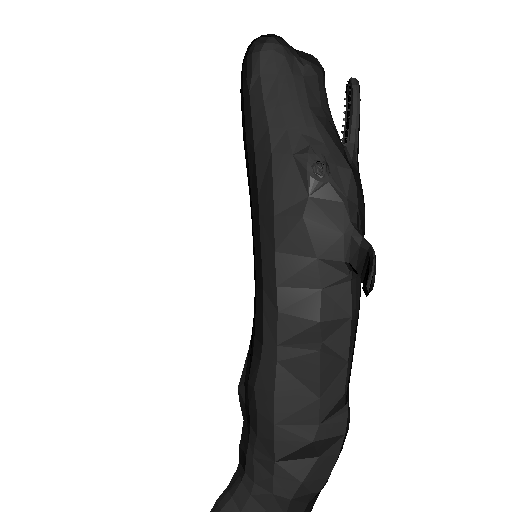
\includegraphics[width=0.8\linewidth]{render.png}
  \caption{Whale model rendered with RenderGirl. 2802 triangles.
    512x512 pixels. 0.421879 seconds. Device used: GeForce GT 650M. FXAA
    off.}
 \label{fig:result1}
\end{figure}

The Core has two interfaces: the wxWidgets interface and the command
line interface. They both work with the same APIs form the core and
are capable of running the raytracer. The wxWidgets interface offers a
GUI which the user can select parameters of the rendering, such as
light color, resolution of the image, several image formats for saving
and options for enable FXAA.

We current have a limitation of only accepting scenes using the OBJ
format, which the core itself will load. In order to be properly
rendered, the model must contains only triangles, otherwise the
software will ignore extra vertices on a face. The Blender plugin
interface aims to reduce the Core responsibilities on this aspect, by
using the already mature infrastructure of Blender for loading and
editing scenes.

Execution for now is restricted to Windows.

With this work, we aim to offer more options for developers of 3D
modeling programas that want to incorporate a GPU raytracer into their
softwares without writing one from scratch. To the best of our
knowledge there's no free software available with the same design
goals.

\subsection{Development Schedule}

Development progress is managed with a scrum-like method using the
Rally Community Software\footnote{Rally Community Edition
 \url{https://rallydev.com/}}. The schedule is divided among
\emph{releases} which are subdivided into \emph{iterations} of two
weeks each. Work is then split into \emph{user stories}, each of them
having a given pontuation, decided at planning phase (usually when the
US is created), each point roughly represents one hour of work. With
this system we aim to properly distribute the workload within the
timeframe we have for the development of the project, and to
prioritize the tasks we deem more important.

The following table provides the timeframe of each release, and the
main features we aim to support at a given point.

\begin{tabular}{ | p{.8cm} | p{1cm} | p{1cm} | p{4cm} |}
  \hline
  Release & Start date & Release date & Major features \\ \hline
  Final Project 1 B & 2015-10-18 & 2015-12-07 & (1)Theoretical base for the raytracer, with clearly defined goals and
                                                general scope of the project. (2)Definition of a method of binary
                                                space partitioning. (3)Definition of a method of anti-aliasing.
                                                (4)Early work on the Blender plugin, with communication between C++ and Python. \\ \hline
  Final Project 2 A & 2015-12-13 & 2016-04-30 & (1)Working software with the features proposed (BVH, anti-aliasing, blender plugin interface).
                                                (2)Updated scope with what was discarded and what was added \\ \hline
  Final Project 2 B & 2016-05-02 & 2016-06-19 & (1)The working software in some stable form (a release branch or tag). (2)Bug fixes.
                                                (3)The documentation for the final user. Including an update version of
                                                the current articles on github page of the project. (4)Results of the work,
                                                with comparative studies and rendergin performance gains.
                                                (5)The final draft of this article. \\ \hline
\end{tabular}

% \section*{Acknowledgments}


\bibliographystyle{sbgames}
\bibliography{references}
\end{document}
